\chapter{Analisi delle sperimentazioni}
\section{Tipo di testing}
Per la fase di testing sono stati selezionati gli algoritmi che sono in grado di rispettare
almeno la seconda delle condizioni poste in principio, risultano perciò esclusi CLA e CSA.\\

Il testing è stato condotto con codice Java tramite la generazione di poligoni convessi
randomici con un numero sempre crescenti di lati $E$ (4 - 30). 
Per ogni $E$ vengono creati 5 politopi differenti e, per ognuno di questi, verranno creati
$E-3$ casi di test, ciascuno con un budget di iperpiani crescente $3 .. E$
per un numero totale di 1729 casi di test sottoposti a ciascun algoritmo.

L'algoritmo utilizzato per la generazione randomica dei poliedri convessi 
è l'algoritmo di Valt, spiegato estensivamente nel rispettivo documento
\cite{ValtrAlgorithm}.

\subsection*{Metriche di valutazione}
Oltre al tempo di esecuzione dei vari algoritmi, per valutarne l'accuratezza si è deciso
di utilizzare l'indice di Jaccard, ampiamente impiegato nella teoria degli insiemi. 
Questo indice misura la somiglianza tra due insiemi calcolando il rapporto tra 
l'intersezione e l'unione degli stessi, ovvero:
 
\[
J(A, B) = \frac{|A \cap B|}{|A \cup B|}
\]

Applicando tale principio ai politopi, si può valutare il rapporto tra il politopo originale 
e quello approssimato. In particolare, l'indice di Jaccard consente di stimare il volume 
eccedente rispetto al volume del politopo originale con valori compresi tra 0 e 1.\\

Dopo aver eseguito il test, i risultati vengono immagazzinati in una tabella csv per poter 
effettuare delle analisi tramite l'utilizzo di librerie Python.


\subsection*{Limiti del testing}
Un limite fondamentale dell'algoritmo di generazione di gusci convessi in due dimensioni 
consiste nel fatto che, all'aumentare del numero di lati del poiliedro generato, 
la forma che questo assumerà sarà sempre più probabilmente simile ad una forma
ben stabilita in questa ricerca di Pavel Valt.\cite{probabilityConvexhull2d}

\pagebreak
\section{Analisi dei dati} 
\label{sec:Analisi dei dati}
I risultati ottenuti evidenziano che gli algoritmi che selezionano gli iperpiani 
per creare l'approssimazione possono generare politopi aperti. In particolare, 
l'algoritmo \textit{LessArea} è quello più incline a produrre politopi di approssimazione aperti, 
fenomeno osservato in 23 casi su un totale di 1729.\\
Anche l'algoritmo \textit{BoxCutting} può occasionalmente generare politopi aperti, 
sebbene questo accada con minore frequenza. 
Grazie alla sua euristica evolutiva nella selezione degli iperpiani, 
sono stati riscontrati solo 7 casi su 1729. Questo comportamento si manifesta principalmente 
in presenza di politopi iniziali con un elevato numero di facce e con budget di iperpiani 
molto limitato.

Le probabilità complessive che si verifichi questo evento risultano tuttavia 
non influenti al fine dell'analisi sulle statistiche ($\leq 1\%$).

Come evidenziato nella tabella \ref{tab:results} i dati risultano essere nettamente a favore di
alcuni algoritmi che riescono ad ottenere dei buoni risultati apportando allo stesso
tempo tempi di esecuzione in media inferiori.

\begin{table}[h] 
    \centering
    \begin{tabular}{|c|c|c|}
        \hline
        Algoritmo & Jaccard Index & Tempo Medio (Millisec) \\
        \hline
        BoxCutting              & 0.90  & 1.67\\
        CuttingEdges            & 0.94  & 0.59\\ 
        CuttingLargerAngle2     & 0.91  & 0.70 \\
        CuttingSmallerAngle2    & 0.48  & 0.69 \\
        DistanceFromG           & 0.69  & 4.00 \\
        LessArea                & 0.74  & 298.76 \\
        \hline
    \end{tabular}
    \caption{Tabella riassuntiva delle prestazioni delle euristiche} 
    \label{tab:results}
\end{table} 

Dato l'elevato costo computazionale dell'euristica LessArea, i seguenti grafici
non conterranno le informazioni inerenti a questo Algoritmo.

\subsection*{Tempi di esecuzione}

\begin{figure}[H]
    \centering
    \begin{minipage}[b]{0.45\textwidth}
        \centering
        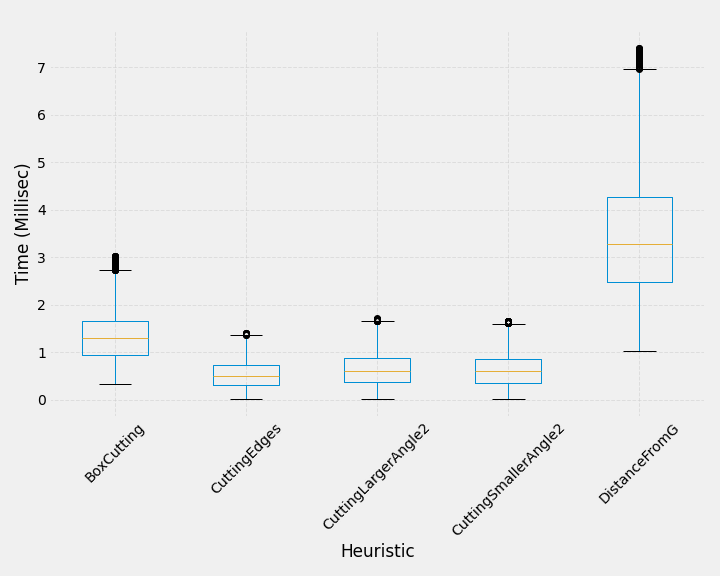
\includegraphics[width=\textwidth]{media/report/bxplt_time.png}
        \caption{boxplot del tempo medio di esecuzione per ciascuna euristica.\\
        }
    \end{minipage}
    \hspace{0.05\textwidth}
    \begin{minipage}[b]{0.45\textwidth}
        \centering
        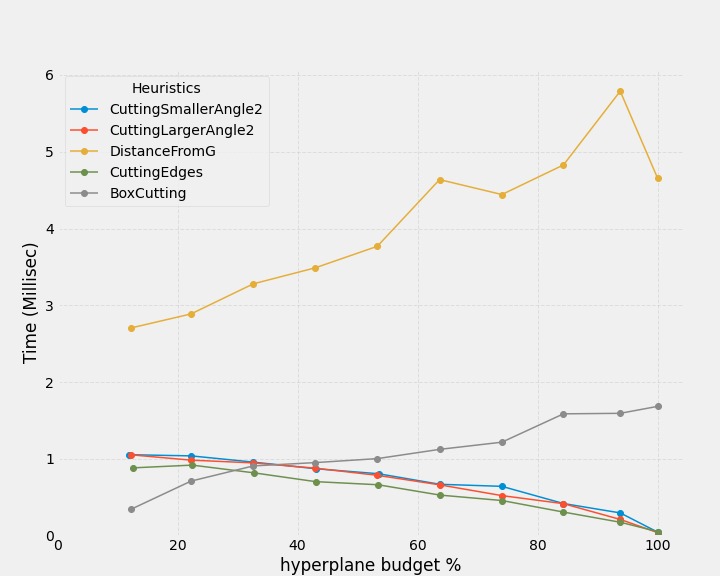
\includegraphics[width=\textwidth]{media/report/Time_plot.png}
        \caption{andamento dei tempi di esecuzione di ciascuna euristica in base al budget di iperpiani $h$.}
        \label{fig: time_h}
    \end{minipage}
\end{figure}

Osservando i tempi medi di esecuzione degli algoritmi si possono discernere due principali
classi di algoritmi, il primo dei quali ha un tempo di esecuzione nettamente inferiore rispetto al secondo.
In particolare dal grafico in Figura \ref*{fig: time_h} si distinguono fra tutti gli algoritmi BoxCutting e CuttingEdge 
che risultano essere più efficienti per differenti budget di iperpiani.

\subsection*{Accuratezza}

\begin{figure}[H]
    \centering
    \begin{minipage}[b]{0.45\textwidth}
        \centering
        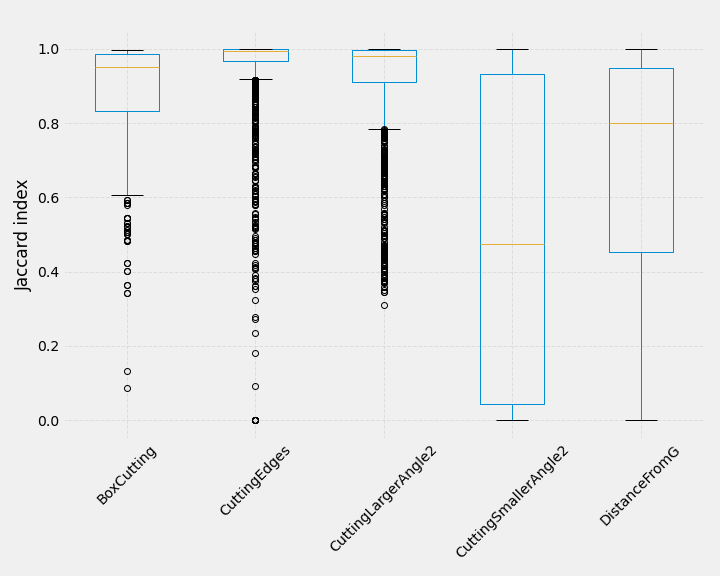
\includegraphics[width=\textwidth]{media/report/bxplt_jaccard.png}
        \caption{boxplot dell'accuratezza del politopo di approssimazione per ciascuna euristica.}
    \end{minipage}
    \hspace{0.05\textwidth}  
    \begin{minipage}[b]{0.45\textwidth}
        \centering
        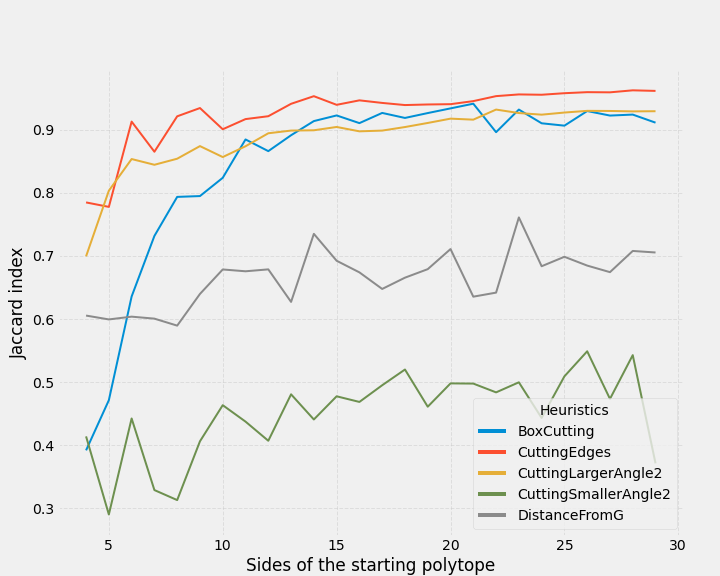
\includegraphics[width=\textwidth]{media/report/Accuracy_plot.png}
        \caption{andamento dell'accuratezza di approssimazione di ciascuna euristica in base al numero di lati del poligono iniziale.}
    \end{minipage}
\end{figure}

I due grafici sovrastanti espongono con quale costanza e quale accuratezza i politopi 
di approssimazione generati dagli algoritmi rappresentino il politopo di partenza.\\
Si può notare inoltre come un gruppo di algoritmi riesca a mantenere una
precisione costantemente piu accurata rispetto ad altri.